%%% TITLE AND AUTHORS %%%%%%%%%%%%%%%%%%%%%%%%%%%%%%%%%%%%%%%%%%%%%%%%%%%%%%%%%

\title[Introduction \& syllabus]{
    Introduction and syllabus \\
    \small{}
}
\author[]{Szymon Talaga and Mikołaj Biesaga} % Your name
\institute[ISS UW]{
    The Robert Zajonc Institute for Social Studies \\ University of Warsaw \\
    \medskip
    \textit{stalaga@uw.edu.pl} \\
    \textit{m.biesaga@uw.edu.pl}
}
\date{2 October 2019} % Date, can be changed to a custom date

%%% SLIDES %%%%%%%%%%%%%%%%%%%%%%%%%%%%%%%%%%%%%%%%%%%%%%%%%%%%%%%%%%%%%%%%%%%%
\frame{\titlepage}

\part[Syllabus]{Syllabus}
\frame{\partpage}

\section[Rules]{Rules of Engagement}
\subsection[Communication]{Communication}
\begin{frame}
    \frametitle{Office Hours, Emails, and Slack}
    \begin{description}[Office Hours:]
        \item[Office Hours:] write us an email or on Slack before coming
        \item[Emails:] the official info will go thorough emails
        \item[Slack:] register at \href{www.slack.com}{www.slack.com}
        \item[Google Drive:] materials and presentations will be posted at \href{https://drive.google.com/a/uw.edu.pl/file/d/1VotLZIEmp4lXnT-NdR0yZ5DDal59FfkI/view?usp=sharing}{Google Drive}
    \end{description}
    \action<visible@+>{\alert{We will try to answer your inquires as soon as possible but do not count on imidiate response, especially before the deadlines.}}
\end{frame}

\subsection[Assessment]{Assessment Criteria}
\begin{frame}
    \frametitle{Assessment Criteria}
    \begin{block}{}
        Final Grade = 30\%$\times$Homeworks + 35\%$\times$Final Exam + 35\%$\times$written report\\
    \end{block}
        \begin{itemize}
        \item Homeworks - 3 written assignments (approximately after weeks 7, 9, and 13)
        \item Final Exam - will cover theoretical material discussed in the classroom (15.01.2019)
        \item Written Report - a research project proposal formulating a research problem that can be addressed with the methods discussed during the course (due to the last class - 22.01.2019)
    \end{itemize}
\end{frame}

\subsection[Attendance]{Attendance}
\begin{frame}
    \frametitle{Attendance}
    \begin{itemize}
        \item You are allowed to miss up to 2 classes without formal excuse
        \item  absence does not exempt from doing homework assignments
    \end{itemize}
    \action<visible@+>{\alert{It is better not to miss classes because this is a relatively challenging course and it will be hard to cover the material from the class at home.}}
\end{frame}

\subsection[Workflow]{Workflow}
\begin{frame}
    \frametitle{Workflow}
    \begin{enumerate}
        \item We will present you with some concepts in the classroom.
        \item You will read about it at home.
        \item We will present you with the working examples in the classroom.
        \item You will try modifying the examples for home assignments.
    \end{enumerate}
    \action<visible@+>{\alert{If you cannot find the answer on Internet you are asking the wrong question.}}
\end{frame}

\part[Introduction]{Introduction}
\frame{\partpage}

\section[CSS]{Computational Social Science}

\begin{frame}
    \frametitle{What is Computational Social Science?}
    \begin{block}{}
        In the most general sense \emph{Computational Social Science} is a data-driven approach which uses computational methods in studying social phenomena.
    \end{block}
    \begin{block}{}
        It is closely related to the field of data science, which can be
        defined as set of theory and practices related to answering research questions
        based on empirical data, including large volumes of unstructured numeric
        and textual data, using the scientific methods, processes and algorithms.
        It sits at the intersection statistics, computer science and mathematics.
    \end{block}
\end{frame}

\begin{frame}{General interest in data science}
    \begin{figure}
    \setbeamertemplate{caption}
    \caption{Growth of Google search}
    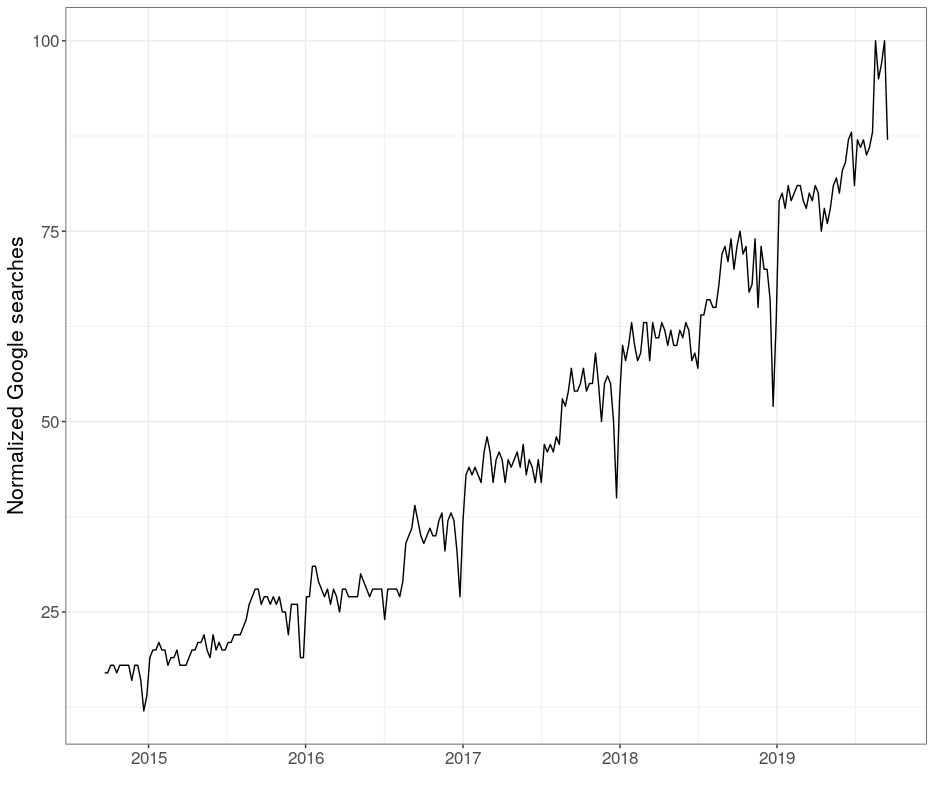
\includegraphics[width = .8\framewidth]{png/ds-searches.png}

    \end{figure}
\end{frame}

\section[Data]{Data}

\subsection[Data Sources]{Data Sources}

\begin{frame}
    \frametitle{Traditional Data Sources}
    \begin{itemize}
        \item What are the traditional data sources for psychologist?
        \item Qualitative and Quantitive
        \item Structured data and unstructured data
        \item What are the new data sources for psychologist?
    \end{itemize}
\end{frame}

\subsection{Webscraping}

\begin{frame}
    \frametitle{Webscraping}
\end{frame}

\subsection{API}

\begin{frame}
    \frametitle{Application Programming Interface}
\end{frame}

\subsection[Data Formats]{Data Formats}

\begin{frame}[fragile]{Data formats}
    \defverbatim[colored]\mycode{%
        \begin{lstlisting}[
            frame=single,
            language=json,
            firstnumber=1,
            basicstyle=\footnotesize\ttfamily
        ]
    persons: [
        { name: "Alice",
          age: 17,
          interests: [
            { name: "sport",
              tags: [
                "physical activity",
                "outdoor"
            ] }
        ] },
        { name: "Bob",
          age: 18,
         interests: [] }
    ] }
        \end{lstlisting}
    }

    \begin{itemize}
        \item Computational studies often entail working with datasets that
        can not be easily represented with traditional data tables typically
        used in psychology and social sciences (respondents in rows, variables in columns).
        \item Usually one has to work with complicated semi-structured nested
        data formats like JSON:
    \end{itemize}
    \mycode
\end{frame}

\begin{frame}{Computational methods\footnote{
    In this class we focuse on the parts written in bold.
}}
\begin{itemize}
    \item \textbf{Extraction of unstructured data from external digital (i.e. web-based)
    sources.}
    \begin{itemize}
        \item \textbf{Webscraping (extraction of data from existing webpages).}
        \item \textbf{Extracting data from web APIs (i.e. Twitter).}
    \end{itemize}
    \item \textbf{Analysis of textual data (natural language processing - NLP).}
    \item Network and relational data analysis.
    \item Working with big datasets (that do not fit into RAM of a single computer).
    In-database computations, distributed computing etc.
    \item Computer simulations.
    \item Online experiments (A/B testing, experiments based on online games etc.).
\end{itemize}
\end{frame}

\begin{frame}{Goal of the class}
\begin{itemize}
    \item In general the practice of data science and computational social science
    requires a lot of technical skills such as computer programming and statistics,
    which can not be taught in a brief one-semester course like this.
    \item However, not everyone in a research project has to be a techie.
    \item But it is necessary that everyone in a team has the basic knowledge
    about modern computational technologies and methods, so everyone shares
    the same language which makes it possible to communicate efficiently regardless
    of difference in background and training.
    \item This class is meant to teach you this language, so you can
    collaborate with technical persons and design computationally-oriented
    studies.
\end{itemize}
\end{frame}

\begin{frame}{General advice}
\begin{itemize}
    \item In this class we do not expect any background in computer science,
    programming etc.
    \item However, it will be relatively difficult, especially for those of you
    who are not particularly tech-savvy.
    \item This is why it is absolutely crucial to try to do all the homework
    we will assign to you, as they are necessary for you to internalize
    the material.
    \item You are allowed to miss up to two classes. However, we really recommend
    to attend all of them, as some parts of the material will build on the
    earlier parts.
\end{itemize}
\end{frame}

%%% LITERATURE %%%%%%%%%%%%%%%%%%%%%%%%%%%%%%%%%%%%%%%%%%%%%%%%%%%%%%%%%%%%%%%%
\begin{frame}{Literature to read}
\nocite{*}
\AtNextBibliography{\footnotesize}
\printbibliography
\end{frame}

\begin{frame}{Closing remarks}
\begin{itemize}
    \item This is the first edition of this course.
    \item Feel free to let us know when something does not work well for you.
    \item This is going to be a challenging course.
    \item \href{www.stackexchange.com}{Stack Exchange}
    \item \href{www.stackoverflow.com}{Stack Overflow}
\end{itemize}
\end{frame}
